\section{A four-tile substitution system}
\label{sec:subst}

Consider the four metatiles, with matching conditions as in
Figure~\ref{fig:tileaclusters}, which are depicted in this section in
the form shown in Figure~\ref{fig:subst}.  Edges $A$ are
\textcolor{\colA}{\textbf{red}}, $B$ are
\textcolor{\colB}{\textbf{blue}}, $X$ are
\textcolor{\colX}{\textbf{green}}, $F$ are
\textcolor{\colF}{\textbf{pink}}, and $L$ are
\textcolor{\colL}{\textbf{gray}}.  Edges are marked with small
geometrical decorations to indicate the signs (outward on the
${}^+$~side, inward on the ${}^-$~side): equilateral triangles
for~$A$, semicircles for~$B$, orthogonal line segments for~$X$, short
slanted line segments for~$F$.  Note that the $A$ and $B$ on $H$ are
the opposite signs to those on $T$, $P$, and $F$.  Also note that the
tiles in this substitution system may not be reflected, only rotated.

\begin{figure}[htp!]
\begin{center}
\begin{tikzpicture}[x=5mm,y=5mm,ultra thick]
  \Ttile{0}{0}{0}{$T$};
  \Htile{0}{4}{-2}{$H$};
  \Ptile{0}{10}{-5}{$P$};
  \Ftile{0}{17}{-8.5}{$F$};
\end{tikzpicture}
\end{center}
\caption{Metatiles $T$, $H$, $P$, and $F$}
\label{fig:subst}
\end{figure}

Later in the argument it is convenient to bisect some tiles~$P$
and~$F$, as shown in Figure~\ref{fig:substbisect}.  We refer to the
edges resulting from the bisection of~$P$ as $P^+$ (in the sub-tile
that has an edge~$B^+$) and $P^-$, coloured
\textcolor{\colP}{\textbf{yellow}} and decorated with a rectangle, and
to the edges resulting from the bisection of $F$ as $G^+$ (in the
sub-tile that has an edge~$B^+$) and $G^-$, coloured
\textcolor{\colG}{\textbf{violet}} and decorated with an obtuse
triangle.  We also refer to the halves with a $B^+$~edge as the upper
halves, and the other halves as the lower halves.  We will show the
following:

\begin{theorem}
\label{thm:subst}
In any tiling by the four metatiles, after such bisection of $P$
and~$F$ metatiles, the metatiles fit together to form larger,
combinatorially equivalent supertiles, thereby forming a substitution
system.  The tiling by the supertiles has the same symmetries as the
tiling by the metatiles.
\end{theorem}

\begin{figure}[htp!]
\begin{center}
\begin{tikzpicture}[x=5mm,y=5mm,ultra thick]
  \Pplus{0}{0}{0}{};
  \Pminus{0}{1.5}{-1.5}{};
  \Fplus{0}{8}{-4}{};
  \Fminus{0}{9.5}{-5.5}{};
\end{tikzpicture}
\end{center}
\caption{Bisection of tiles $P$ and $F$}
\label{fig:substbisect}
\end{figure}

The bisection of tiles is not strictly necessary, in that the
bisecting lines can be arbitrary curves---and, in particular, can go
entirely along one side or other of the $F$ or $P$ tiles (keeping the
same end points), effectively allocating an entire tile to one of
two neighbouring supertiles.  However, the bisected tiles are convenient
for proving that the supertiles obey matching rules equivalent to those
of the original tiles.  In particular, bisection causes adjacencies
between supertiles to be more clearly encoded in 
the boundaries of the supertiles themselves, without also relying on
information about forced tiles that are not part of the supertiles.
In some situations it may be more useful to assign whole tiles to supertiles
at every level of substitution, with no bisection.  
For example, these whole tiles may be more convenient for analyzing sizes
or growth rates of patches in the inflation process.
If needed, we can
define a symmetry-preserving bijection between the supertiles
shown here and any alternative choice of supertiles that avoids bisection.

Diagrams for analysis of cases should be interpreted as follows.
There are some unnumbered tiles that define the case being considered,
then some numbered tiles that are forced in the sequence given by
their numbers.  If it is then necessary to split into multiple cases,
the position at which multiple choices of tile must be considered is
marked on the diagram with a filled circle, and there are then
separate diagrams for each choice (on which the previous forced tiles
are now unnumbered, but newly forced tiles are numbered).

The configuration in Figure~\ref{fig:PP}, referred to as~$PP$, often
appears in the case
analysis; the two adjoining copies of~$P$ in the same orientation
force a contradiction because nothing fits at the marked point.
Subsequently, when identifying forced tiles, as well as considering a
tile as forced when it is the only one that would fit in a given place
consistent with the matching conditions, we also consider a tile as
forced when the only alternative consistent with the matching
conditions would be to place a $P$~tile in a way that produces this~$PP$ 
configuration. 

\begin{figure}[htp!]
\begin{center}
\begin{tikzpicture}[x=5mm,y=5mm,ultra thick]
  \Ptile{60}{0}{0}{};
  \Ptile{60}{1}{4}{};
  \Htile{0}{2}{0}{1};
  \Htile{0}{3}{4}{2};
  \markpt{4}{3};
\end{tikzpicture}
\end{center}
\caption{A common impossible configuration, referred to as $PP$}
\label{fig:PP}
\end{figure}

\subsection{Cases involving $T$}

The two $A^-$ edges of~$T$ must be adjacent to the $A^+$ edge of~$H$,
while the $B^+$~edge of~$T$ may be adjacent to either of the
$B^-$~edges of~$H$.  Thus we have two cases for the configuration
around a $T$~tile, which we refer to as $T1$ and $T2$
(Figure~\ref{fig:T1T2}).  As explained in the captions to this and
subsequent figures, a sequence of deductions shows that any~$T$ in a
tiling must occur in case~$T1PF$ (Figure~\ref{fig:T1PF}).

\begin{figure}[htp!]
\begin{center}
\subfloat[Case $T1$]{%
  \begin{tikzpicture}[x=5mm,y=5mm,ultra thick]
  \Ttile{0}{0}{0}{};
  \Htile{-60}{-1}{0}{};
  \Htile{60}{4}{-1}{};
  \Htile{60}{-1}{0}{};
  \markpt{-1}{0};
  \markpt{4}{-1};
  \markpt{0}{4};
\end{tikzpicture}%
} \qquad \subfloat[Case $T2$]{%
\begin{tikzpicture}[x=5mm,y=5mm,ultra thick]
  \Ttile{0}{0}{0}{};
  \Htile{-60}{-1}{0}{};
  \Htile{60}{4}{-1}{};
  \Htile{-60}{-5}{5}{};
  \markpt{-1}{0};
  \markpt{4}{-1};
  \markpt{0}{4};
\end{tikzpicture}%
}%
\end{center}
\caption{Cases $T1$ and $T2$.  Consider the three marked places in
  each of $T1$ and~$T2$.  These can be filled with either $P$ or~$H$.
  On a side of the figure where there are two $B^-$~edges, the marked
  place cannot be filled with~$H$, because that would result in a
  $60^\circ$~angle between two $B^-$~edges, which cannot be filled.
  So both those sides must have $P$~in the marked place, while the
  third side may have $H$ (oriented to avoid such a $60^\circ$~angle
  between two $B^-$~edges; subsequently, when the same situation
  arises, we just consider the orientation of the~$H$ to be forced
  without further comment) or~$P$.  This results in four cases, which
  we call $T1P$ (Figure~\ref{fig:T1P}), $T2P$ (Figure~\ref{fig:T2P}),
  $T1H$ (Figure~\ref{fig:T1H}) and $T2H$ (Figure~\ref{fig:T2H}), and
  we proceed to draw further forced tiles in each of those cases.}
\label{fig:T1T2}
\end{figure}

\begin{figure}[htp!]
\begin{center}
\begin{tikzpicture}[x=5mm,y=5mm,ultra thick]
  \Ttile{0}{0}{0}{};
  \Htile{-60}{-1}{0}{};
  \Htile{60}{4}{-1}{};
  \Htile{60}{-1}{0}{};
  \Ptile{60}{4}{-5}{};
  \Ptile{180}{4}{4}{};
  \Ptile{120}{-1}{-2}{};
  \Ftile{60}{5}{-1}{1};
  \Ftile{-60}{2}{8}{2};
  \Ftile{180}{-1}{5}{3};
  \Ftile{60}{-7}{2}{4};
  \markpt{-1}{-1};
\end{tikzpicture}
\end{center}
\caption{Case $T1P$.  The marked place can be filled with $F$ or~$P$,
  resulting in cases we call $T1PF$ (Figure~\ref{fig:T1PF}) and $T1PP$
  (Figure~\ref{fig:T1PP}).}
\label{fig:T1P}
\end{figure}

\begin{figure}[htp!]
\begin{center}
\begin{tikzpicture}[x=5mm,y=5mm,ultra thick]
  \Ttile{0}{0}{0}{};
  \Htile{-60}{-1}{0}{};
  \Htile{60}{4}{-1}{};
  \Htile{-60}{-5}{5}{};
  \Ptile{60}{4}{-5}{};
  \Ptile{-60}{-5}{4}{};
  \Ptile{180}{4}{4}{};
  \Ptile{0}{-7}{7}{1};
  \Ftile{120}{-5}{3}{2};
  \Htile{-120}{-5}{2}{3};
  \Htile{120}{-5}{2}{4};
  \Ftile{-60}{-1}{-1}{5};
  \Ptile{0}{-5}{-3}{6};
  \Ttile{180}{-6}{2}{7};
  \Htile{-120}{-10}{3}{8};
  \Ptile{0}{-10}{-2}{9};
  \markpt{-4}{-4};
\end{tikzpicture}
\end{center}
\caption{Case $T2P$, eliminated because $PP$ occurs at the marked point.}
\label{fig:T2P}
\end{figure}

\begin{figure}[htp!]
\begin{center}
\begin{tikzpicture}[x=5mm,y=5mm,ultra thick]
  \Ttile{0}{0}{0}{};
  \Htile{-60}{-1}{0}{};
  \Htile{60}{4}{-1}{};
  \Htile{60}{-1}{0}{};
  \Ptile{60}{4}{-5}{};
  \Ptile{180}{4}{4}{};
  \Htile{180}{-1}{0}{};
  \Ttile{-120}{-1}{-1}{1};
  \Htile{-60}{-2}{-4}{2};
  \Ptile{60}{3}{-9}{3};
  \markpt{5}{-5};
\end{tikzpicture}
\end{center}
\caption{Case $T1H$, eliminated because $PP$ occurs at the marked point.}
\label{fig:T1H}
\end{figure}

\begin{figure}[htp!]
\begin{center}
\begin{tikzpicture}[x=5mm,y=5mm,ultra thick]
  \Ttile{0}{0}{0}{};
  \Htile{-60}{-1}{0}{};
  \Htile{60}{4}{-1}{};
  \Htile{-60}{-5}{5}{};
  \Ptile{60}{4}{-5}{};
  \Ptile{-60}{-5}{4}{};
  \Htile{180}{1}{8}{};
  \Ttile{120}{4}{4}{1};
  \Htile{60}{5}{3}{2};
  \Ptile{60}{5}{-1}{3};
  \markpt{6}{-1};
\end{tikzpicture}
\end{center}
\caption{Case $T2H$, eliminated because $PP$ occurs at the marked point.}
\label{fig:T2H}
\end{figure}

\begin{figure}[htp!]
\begin{center}
\begin{tikzpicture}[x=5mm,y=5mm,ultra thick]
  \Ttile{0}{0}{0}{};
  \Htile{-60}{-1}{0}{};
  \Htile{60}{4}{-1}{};
  \Htile{60}{-1}{0}{};
  \Ptile{60}{4}{-5}{};
  \Ptile{180}{4}{4}{};
  \Ptile{120}{-1}{-2}{};
  \Ftile{60}{5}{-1}{};
  \Ftile{-60}{2}{8}{};
  \Ftile{180}{-1}{5}{};
  \Ftile{60}{-7}{2}{};
  \Ftile{-60}{-1}{-1}{};
  \Ftile{180}{8}{-7}{1};
\end{tikzpicture}
\end{center}
\caption{Case $T1PF$.  Any $T$ in a tiling must occur in this case.
  Bisecting the $P$ and~$F$ tiles in that case produces the
  configuration of Figure~\ref{fig:Hsuper}, which we call~$H'$ and
  which combinatorially acts like~$H$ (with the edge segments
  indicated marked for matching conditions) in a tiling along with
  configurations $T'$, $P'$, and~$F'$.}
\label{fig:T1PF}
\end{figure}

\begin{figure}[htp!]
\begin{center}
\begin{tikzpicture}[x=5mm,y=5mm,ultra thick]
  \Ttile{0}{0}{0}{};
  \Htile{-60}{-1}{0}{};
  \Htile{60}{4}{-1}{};
  \Htile{60}{-1}{0}{};
  \Ptile{60}{4}{-5}{};
  \Ptile{180}{4}{4}{};
  \Ptile{120}{-1}{-2}{};
  \Ftile{60}{5}{-1}{};
  \Ftile{-60}{2}{8}{};
  \Ftile{180}{-1}{5}{};
  \Ftile{60}{-7}{2}{};
  \Ptile{-60}{-1}{-1}{};
  \Ftile{-120}{5}{-5}{1};
  \Htile{0}{6}{-5}{2};
  \Htile{-120}{6}{-5}{3};
  \Ttile{-60}{7}{-6}{4};
  \Htile{0}{10}{-10}{5};
  \Ptile{120}{15}{-10}{6};
  \Ptile{120}{11}{-5}{7};
  \markpt{11}{-4};
\end{tikzpicture}
\end{center}
\caption{Case $T1PP$, eliminated because $PP$ occurs at the marked point.}
\label{fig:T1PP}
\end{figure}

\FloatBarrier

\subsection{Cases with $H$ not adjacent to $T$}

Any $H$ not adjacent to a $T$~tile must have a $P$~tile adjacent to
its $A^+$ edge, while the $B^-$ edges may each be adjacent to $P$
or~$F$.  This results in four cases, which we call $HPP$
(Figure~\ref{fig:HPP}), $HPF$ (Figure~\ref{fig:HPF}), $HFP$
(Figure~\ref{fig:HFP}), and $HFF$ (Figure~\ref{fig:HFF}), and we
proceed to draw further forced tiles in each of those cases, with
consequences explained in the captions to those figures.

\begin{figure}[htp!]
\begin{center}
\begin{tikzpicture}[x=5mm,y=5mm,ultra thick]
  \Htile{0}{0}{0}{};
  \Ptile{60}{-2}{0}{};
  \Ptile{120}{5}{0}{};
  \Ptile{0}{1}{-1}{};
  \Ftile{60}{-1}{4}{1};
  \Ftile{-60}{5}{1}{2};
  \Ftile{180}{2}{-2}{3};
\end{tikzpicture}
\end{center}
\caption{Case $HPP$.  Bisecting the $P$ tiles and removing the forced
  $F$~tiles produces the configuration of Figure~\ref{fig:Tsuper},
  which we call~$T'$ and which combinatorially acts like~$T$ (with the
  edge segments indicated marked for matching conditions) in a tiling
  with the other supertiles.  Although the forced $F$~tiles are not
  included in~$T'$, the fact that they are forced will be used in the
  proof that the supertiles must follow the matching conditions where
  they are adjacent to each other.}
\label{fig:HPP}
\end{figure}

\begin{figure}[htp!]
\begin{center}
\begin{tikzpicture}[x=5mm,y=5mm,ultra thick]
  \Htile{0}{0}{0}{};
  \Ptile{60}{-2}{0}{};
  \Ptile{120}{5}{0}{};
  \Ftile{0}{1}{-1}{};
  \Ftile{-120}{7}{2}{1};
  \Ftile{60}{-1}{4}{2};
  \Htile{60}{5}{2}{3};
  \Ftile{180}{5}{7}{4};
\end{tikzpicture}
\end{center}
\caption{Case $HPF$.  The second $H$ cannot be adjacent to a~$T$; it
  must thus itself be in case $HFP$ or~$HFF$, and each of those cases
  turns out to force the $H$~tile in case~$HPF$.}
\label{fig:HPF}
\end{figure}

\begin{figure}[htp!]
\begin{center}
\begin{tikzpicture}[x=5mm,y=5mm,ultra thick]
  \Htile{0}{0}{0}{};
  \Ptile{60}{-2}{0}{};
  \Ftile{120}{5}{0}{};
  \Ptile{0}{1}{-1}{};
  \Ftile{0}{-4}{6}{1};
  \Ftile{180}{2}{-2}{2};
  \Ftile{-60}{-7}{4}{3};
  \Htile{-60}{-7}{5}{4};
  \Ptile{0}{-9}{7}{5};
\end{tikzpicture}
\end{center}
\caption{Case $HFP$.  Bisecting the $P$ and~$F$ tiles produces the
  configuration of Figure~\ref{fig:Psuper}, which we call $P'$ and
  which combinatorially acts like~$P$ (with the edge segments
  indicated marked for matching conditions) in a tiling with the other
  supertiles.}
\label{fig:HFP}
\end{figure}

\begin{figure}[htp!]
\begin{center}
\begin{tikzpicture}[x=5mm,y=5mm,ultra thick]
  \Htile{0}{0}{0}{};
  \Ptile{60}{-2}{0}{};
  \Ftile{120}{5}{0}{};
  \Ftile{0}{1}{-1}{};
  \Ftile{-120}{7}{2}{1};
  \Ftile{0}{-4}{6}{2};
  \Ftile{180}{2}{-2}{3};
  \Ftile{-60}{-7}{4}{4};
  \Htile{-60}{-7}{5}{5};
  \Ptile{0}{-9}{7}{6};
\end{tikzpicture}
\end{center}
\caption{Case $HFF$.  Bisecting the $P$ and~$F$ tiles produces the
  configuration of Figure~\ref{fig:Fsuper}, which we call $F'$ and
  which combinatorially acts like~$F$ (with the edge segments
  indicated marked for matching conditions) in a tiling with the other
  supertiles.}
\label{fig:HFF}
\end{figure}

\FloatBarrier

\subsection{The supertiles}

\begin{figure}[htp!]
\begin{center}
\begin{tikzpicture}[x=5mm,y=5mm,ultra thick]
  \Htile{0}{0}{0}{};
  \Pminus{60}{-1}{0}{};
  \Pplus{120}{5}{0}{};
  \Pplus{0}{1}{-1}{};
  \markpt{1}{-1};
  \markpt{5}{0};
  \markpt{0}{4};
  \vctxt{5}{-3}{$A^-_2$};
  \vctxt{4}{3}{$A^-_2$};
  \vctxt{-2}{3}{$B^+_2$};
  \Ttile{0}{10}{-5}{$T$};
\end{tikzpicture}
\end{center}
\caption{Supertile $T'$, alongside corresponding $T$}
\label{fig:Tsuper}
\end{figure}

\begin{figure}[htp!]
\begin{center}
\begin{tikzpicture}[x=5mm,y=5mm,ultra thick]
  \Ttile{0}{0}{0}{};
  \Htile{-60}{-1}{0}{};
  \Htile{60}{4}{-1}{};
  \Htile{60}{-1}{0}{};
  \Pplus{60}{4}{-5}{};
  \Pplus{180}{4}{4}{};
  \Pminus{120}{-1}{-1}{};
  \Fplus{60}{5}{-1}{};
  \Fminus{-60}{2}{7}{};
  \Fplus{180}{-1}{5}{};
  \Fminus{60}{-6}{2}{};
  \Fplus{-60}{-1}{-1}{};
  \Fminus{180}{7}{-6}{};
  \markpt{-6}{2};
  \markpt{-1}{-2};
  \markpt{3}{-6};
  \markpt{7}{-6};
  \markpt{6}{-1};
  \markpt{6}{3};
  \markpt{2}{7};
  \markpt{-2}{6};
  \markpt{-6}{6};
  \vctxt{-4}{0}{$A^+_2$};
  \vctxt{1}{-5}{$X^-_2$};
  \vctxt{6}{-8}{$X^+_2$};
  \vctxt{6}{-3}{$B^-_2$};
  \vctxt{7}{1}{$X^-_2$};
  \vctxt{4}{6}{$X^+_2$};
  \vctxt{0}{7}{$B^-_2$};
  \vctxt{-5}{7}{$X^-_2$};
  \vctxt{-7}{4}{$X^+_2$};
  \Htile{60}{14}{-7}{$H$};
\end{tikzpicture}
\end{center}
\caption{Supertile $H'$, alongside corresponding $H$}
\label{fig:Hsuper}
\end{figure}

\begin{figure}[htp!]
\begin{center}
\begin{tikzpicture}[x=5mm,y=5mm,ultra thick]
  \Htile{0}{0}{0}{};
  \Ptile{60}{-2}{0}{};
  \Fplus{120}{5}{0}{};
  \Pplus{0}{1}{-1}{};
  \Fminus{0}{-3}{5}{};
  \Fminus{180}{1}{-1}{};
  \Fplus{-60}{-7}{4}{};
  \Htile{-60}{-7}{5}{};
  \Pminus{0}{-8}{6}{};
  \markpt{-7}{4};
  \markpt{-7}{3};
  \markpt{-3}{-1};
  \markpt{1}{-1};
  \markpt{5}{0};
  \markpt{5}{1};
  \markpt{1}{5};
  \markpt{-3}{5};
  \vctxt{-8}{4}{$L_2$};
  \vctxt{-6}{1}{$X^-_2$};
  \vctxt{0}{-2}{$X^+_2$};
  \vctxt{5}{-3}{$A^-_2$};
  \vctxt{6}{0}{$L_2$};
  \vctxt{4}{3}{$X^-_2$};
  \vctxt{-1}{6}{$X^+_2$};
  \vctxt{-6}{7}{$B^+_2$};
  \Ptile{0}{10}{-5}{$P$};
\end{tikzpicture}
\end{center}
\caption{Supertile $P'$, alongside corresponding $P$}
\label{fig:Psuper}
\end{figure}

\begin{figure}[htp!]
\begin{center}
\begin{tikzpicture}[x=5mm,y=5mm,ultra thick]
  \Htile{0}{0}{0}{};
  \Ptile{60}{-2}{0}{};
  \Fplus{120}{5}{0}{};
  \Fplus{0}{1}{-1}{};
  \Fminus{-120}{6}{2}{};
  \Fminus{0}{-3}{5}{};
  \Fminus{180}{1}{-1}{};
  \Fplus{-60}{-7}{4}{};
  \Htile{-60}{-7}{5}{};
  \Pminus{0}{-8}{6}{};
  \markpt{-7}{4};
  \markpt{-7}{3};
  \markpt{-3}{-1};
  \markpt{1}{-1};
  \markpt{2}{-2};
  \markpt{6}{-2};
  \markpt{5}{2};
  \markpt{1}{5};
  \markpt{-3}{5};
  \vctxt{-8}{4}{$L_2$};
  \vctxt{-6}{1}{$X^-_2$};
  \vctxt{-0.5}{-2}{$X^+_2$};
  \vctxt{1.25}{-2}{$L_2$};
  \vctxt{5}{-3}{$X^-_2$};
  \vctxt{7}{0}{$F^+_2$};
  \vctxt{4}{3}{$F^-_2$};
  \vctxt{-1}{6}{$X^+_2$};
  \vctxt{-6}{7}{$B^+_2$};
  \Ftile{0}{10}{-5}{$F$};
\end{tikzpicture}
\end{center}
\caption{Supertile $F'$, alongside corresponding $F$}
\label{fig:Fsuper}
\end{figure}

The previous arguments have shown that every $H$ or $T$ tile appears
in a configuration corresponding to the supertiles $T'$, $H'$, $P'$ or
$T'$.  We now provide more detailed rules for allocating each $H$ or
$T$ tile, and, after bisecting all $P$ and $F$ tiles, each half of
such a tile, to groupings of tiles, such that each tile is allocated
to exactly one grouping, the groupings all have the form of one of the
supertiles, all symmetries of the original tiling are also symmetries
of the tiling by supertiles (this property follows immediately from
the form of the rules, which do not involve any arbitrary choices that
could break symmetry), and the supertiles adjoin each other in
accordance with the matching conditions indicated ($A^+_2$ adjoining
$A^-_2$, $B^+_2$ adjoining $B^-_2$, $X^+_2$ adjoining $X^-_2$, $F^+_2$
adjoining $F^-_2$, and $L_2$ adjoining $L_2$).

\begin{itemize}
  \item Each $T$ tile is allocated to a $H'$~supertile, along with all
    the $H$~tiles adjacent to that $T$.
  \item Each $H$ tile in case $HPP$ is allocated to a $T'$~supertile.
  \item Each $H$ tile in case $HFP$ is allocated to a $P'$~supertile,
    along with the $H$~tile in case~$HPF$ shown in
    Figure~\ref{fig:HFP}.
  \item Each $H$ tile in case~$HFF$ is allocated to an $F'$~supertile,
    along with the $H$~tile in case~$HPF$ shown in
    Figure~\ref{fig:HFF}.
  \item Each $H$ tile in case $HPF$ was allocated to a supertile by
    exactly one of the previous two rules.
  \item Each half of a $P$ tile, and the upper half of each $F$~tile,
    is adjacent to exactly one $H$~tile along its $A^-$ or $B^+$~edge,
    and is allocated to the same supertile as that $H$~tile.  (Where
    both halves are allocated to the same supertile, the bisection
    isn't shown in the diagrams of the supertiles, to simplify those
    diagrams.)
  \item It remains to allocate the lower halves of $F$~tiles.  Each
    such lower half has a $X^-$~edge between a $L$~edge and a
    $F^+$~edge; it is allocated to the same supertile as the $H$~tile
    adjacent to that $X^-$ edge.  For this allocation rule to be
	well defined, we need to show that this $X^-$ edge is indeed
    adjacent to a $H$~tile.  The only other possibility not violating
    the matching rules would be adjacency to another $F$~tile, as
    shown in Figure~\ref{fig:FF}, but nothing fits at the marked point
    without violating the matching rules, so that cannot occur.
\end{itemize}

The $X^-$ edge referenced in the last allocation rule cannot be
adjacent to any of the exposed $X^+$~edges of $H$~tiles in supertiles
$T'$, $P'$ or~$F'$ without violating the matching rules.  Thus all
lower halves of $F$~tiles are the ones that appear on the diagrams of
the supertiles, and we have shown that the tiling is partitioned into
the supertiles.

\begin{figure}[htp!]
\begin{center}
\begin{tikzpicture}[x=5mm,y=5mm,ultra thick]
  \Ftile{0}{0}{0}{};
  \Ftile{180}{7}{-4}{};
  \markpt{5}{-2};
\end{tikzpicture}
\end{center}
\caption{Impossible adjacency of two $F$ tiles}
\label{fig:FF}
\end{figure}

We now show that the supertiles adjoin each other in accordance with
the matching conditions indicated.  First, we examine $P^+$~edges
(appearing in $A^-_2$ and~$B^-_2$) and $P^-$~edges (appearing in
$A^+_2$ and~$B^+_2$).  $B^-_2$ and~$A^+_2$ appear only in~$H'$, where
their $P^+$ and~$P^-$~edges cannot meet without tiles intersecting.
So $B^-_2$ can only join to~$B^+_2$ and $A^+_2$ can only join to~$A^-_2$.

Next we show that the converse holds: $A^-_2$ can only join to~$A^+_2$
and $B^+_2$ can only join to~$B^-_2$.  For a contradiction, suppose
that the $P^+$ and $P^-$ edges in some $A^-_2$ and~$B^+_2$ are joined.
If the $B^+_2$ comes from a $P'$~supertile, then that $P^-$ bisects
tile~5 in case~$HFP$.  Adjacent tiles 5 and~1 in that configuration
both have $B^+$~edges, which must both be adjacent to $H$~tiles; those
$H$~tiles are adjacent to each other, which can only occur in a
supertile~$H'$, which does not have an $A^-_2$~edge.  The same
argument applies in the case of an $F'$~supertile, considering tiles 6
and~2 in case~$HFF$.  If the~$P^+$ in an~$A^-_2$ from~$P'$ is joined
to a~$B^+_2$, a similar argument applies (considering tile 2 and an
adjacent unnumbered tile in case~$HFP$).  So the only remaining case
would be if both edges come from supertile~$T'$, but that is
inconsistent with the $F$~tiles forced in case~$HPP$.

Having shown that $A^+_2$, $A^-_2$, $B^+_2$, and $B^-_2$ must meet the
matching conditions for the supertiles, now note that the only $X^+$
and $X^-$ edges on the boundaries of the supertiles that are not part
of $A^+_2$, $A^-_2$, $B^+_2$ or $B^-_2$ are those forming part of
$F^+_2$ and~$F^-_2$.  Thus it follows that $F^+_2$ and~$F^-_2$ must
also adjoin each other.  The only remaining $G^+$ and~$G^-$ edges of
the tiles are then those that form $X^-_2$ and $X^+_2$ edges of the
supertiles, so those also match, and the remaining $L$~edges
form~$L_2$, so those also match.

To show that the supertiles are fully combinatorially equivalent to
the original tiles, one more thing must be checked: that the same
combinations of supertiles fit together at vertices as combinations of
tiles fit together at vertices.  Each supertile has been drawn with a
copy of the corresponding tile alongside it, in a corresponding
orientation.  By inspection, if you take any class of edges of the
tiles, including both sides of the edge (for example, $A^+$ and
$A^-$), and take any line segment in the corresponding edges of the
supertiles, the (directed) angle between the (directed) edges in the
tile and in the supertile is consistent across all the diagrams.

This consistency of angles between edges of tiles and of supertiles
means that the angles at vertices of supertiles around a point, each
consecutive pair having matching edges, add up to the same amount as
the corresponding angles for the corresponding tiles (an angle at a
vertex of a supertile equals the angle at the corresponding vertex of
the corresponding tile, plus the difference between the
tile--supertile angles for the two edges, and those differences cancel
when adding up around the point).

So the supertiles are combinatorially equivalent to the tiles, and thus
the above arguments apply inductively to ensure that the composition
of tiles into supertiles may be applied $n$~times for all~$n$.  Since
the radius of a ball contained in the supertiles goes to infinity
with~$n$ (and this does not depend on how the bisection of supertiles
is defined geometrically, although it may be easier to see if an
alternative choice of supertiles is made at this stage that does not
involve bisecting tiles), and the tilings by supertiles have all the
symmetries of the original tiling, it follows that the original tiling
cannot have a translation as a symmetry.  Furthermore, the
substitution structure implies that the metatiles tile arbitrarily
large finite regions of the plane, and hence the whole plane.
